\section{Advanced Topics}

\subsection[OO]{Object orientation}

\begin{frame}[fragile]
  \frametitle{Polymorphism}
  \begin{block}{the concept}
    \begin{itemize}
    \item objects actually have multiple types concurrently
    \item and can be used as any of them
    \end{itemize}
  \end{block}
  \begin{multicols}{2}
    \begin{cppcode*}{gobble=2}
      Polygon *p = new Polygon();

      int f(Drawable *d) {...};
      f(p);  //ok

      try {
        throw *p;
      } catch (Shape e) {
        // will be caught
      }
    \end{cppcode*}
    \columnbreak
    \center
    \begin{tikzpicture}[node distance=1.5cm]
      \classbox{Drawable}{}
      \classbox[below of=Drawable]{Shape}{}
      \classbox[below of=Shape]{Polygon}{}
      \draw[very thick,->] (Polygon) -- (Shape);
      \draw[very thick,->] (Shape) -- (Drawable);
    \end{tikzpicture}
  \end{multicols}
\end{frame}


\begin{frame}[fragile]
  \frametitle{Inheritance privacy and polymorphism}
  \begin{block}{Only public inheritance is visible to code outside the class}
    \begin{itemize}
    \item private and protected are not
    \item this may restrict usage of polymorphism
    \end{itemize}
  \end{block}
  \begin{multicols}{2}
    \begin{cppcode*}{gobble=2}
      Polygon *p = new Polygon();

      int f(Drawable *d) {...};
      f(p);  // Not ok anymore

      try {
        throw *p;
      } catch (Shape e) {
        // ok, will be caught
      }
    \end{cppcode*}
    \columnbreak
    \center
    \begin{tikzpicture}[node distance=1.5cm]
      \classbox{Drawable}{}
      \classbox[below of=Drawable]{Shape}{}
      \classbox[below of=Shape]{Polygon}{}
      \draw[very thick,->] (Polygon) -- (Shape) node[midway,right] {public};
      \draw[very thick,->] (Shape) -- (Drawable) node[midway,right] {private};
    \end{tikzpicture}
  \end{multicols}
\end{frame}

\begin{frame}[fragile]
  \frametitle{Method overloading}
  \begin{block}{the problem}
    \begin{itemize}
    \item a given method of the parent can be overloaded in a child
    \item but which one is called ?
    \end{itemize}
  \end{block}
  \begin{multicols}{2}
    \begin{cppcode*}{gobble=2}
      Polygon *p = new Polygon();
      p->draw(); // ?
      
      Shape* s = p;
      s->draw(); // ?
    \end{cppcode*}
    \columnbreak
    \center
    \begin{tikzpicture}[node distance=1.5cm]
      \classbox{Drawable}{
        void draw();
      }
      \classbox[below of=Drawable]{Shape}{}
      \classbox[below of=Shape]{Polygon}{
        void draw();
      }
      \draw[very thick,->] (Polygon) -- (Shape);
      \draw[very thick,->] (Shape) -- (Drawable);
    \end{tikzpicture}
  \end{multicols}
\end{frame}


\begin{frame}[fragile]
  \frametitle{Virtual methods}
  \begin{block}{the concept}
    \begin{itemize}
    \item methods can be declared {\it virtual}
    \item for these, the most precise object is always considered
    \item for others, the type of the variable decides
    \end{itemize}
  \end{block}
  \pause
  \begin{multicols}{2}
    \begin{cppcode*}{gobble=2}
      Polygon *p = new Polygon();
      p->draw(); // Polygon.draw
      
      Shape* s = p;
      s->draw(); // Drawable.draw
    \end{cppcode*}
    \columnbreak
    \center
    \begin{tikzpicture}[node distance=1.5cm]
      \classbox{Drawable}{
        void draw();
      }
      \classbox[below of=Drawable]{Shape}{}
      \classbox[below of=Shape]{Polygon}{
        void draw();
      }
      \draw[very thick,->] (Polygon) -- (Shape);
      \draw[very thick,->] (Shape) -- (Drawable);
    \end{tikzpicture}
  \end{multicols}    
\end{frame}

\begin{frame}[fragile]
  \frametitle{Virtual methods}
  \begin{block}{the concept}
    \begin{itemize}
    \item methods can be declared {\it virtual}
    \item for these, the most precise object is always considered
    \item for others, the type of the variable decides
    \end{itemize}
  \end{block}
  \begin{multicols}{2}
    \begin{cppcode*}{gobble=2}
      Polygon *p = new Polygon();
      p->draw(); // Polygon.draw
      
      Shape* s = p;
      s->draw();  // Polygon.draw
    \end{cppcode*}
    \columnbreak
    \center
    \begin{tikzpicture}[node distance=1.5cm]
      \classbox{Drawable}{
        virtual void draw();
      }
      \classbox[below of=Drawable]{Shape}{}
      \classbox[below of=Shape]{Polygon}{
        void draw();
      }
      \draw[very thick,->] (Polygon) -- (Shape);
      \draw[very thick,->] (Shape) -- (Drawable);
    \end{tikzpicture}
  \end{multicols}    
\end{frame}

\begin{frame}[fragile]
  \frametitle{Pure Virtual methods}
  \begin{block}{Concept}
    \begin{itemize}
    \item methods that exist but are not implemented
      \item marked by an ``{\it = 0}'' in the declaration
    \item makes their class abstract
    \item an object can only be instantiated for a non abstract class
    \end{itemize}
  \end{block}
  \pause
  \begin{multicols}{2}
    \begin{cppcode*}{gobble=2}
      // Error : abstract class
      Shape *s = new Shape();

      // ok, draw has been implemented
      Polygon *p = new Polygon();
      
      // Shape type still usable
      Shape* s = p;
      s->draw();
    \end{cppcode*}
    \columnbreak
    \center
    \begin{tikzpicture}[node distance=1.5cm]
      \classbox{Drawable}{
        virtual void draw() = 0;
      }
      \classbox[below of=Drawable]{Shape}{}
      \classbox[below of=Shape]{Polygon}{
        void draw();
      }
      \draw[very thick,->] (Polygon) -- (Shape);
      \draw[very thick,->] (Shape) -- (Drawable);
    \end{tikzpicture}
  \end{multicols}
\end{frame}

\begin{frame}[fragile]
  \frametitle{Pure Abtract Class aka Interface}
  \begin{block}{Definition of pure abstract class}
    \begin{itemize}
    \item a class that has
      \begin{itemize}
        \item no data member
        \item all its methods pure virtual
      \end{itemize}
    \item the equivalent of an Interface in Java
    \end{itemize}
  \end{block}
  \begin{multicols}{2}
    \begin{cppcode*}{gobble=2}
      struct Drawable {
        virtual void draw() = 0;
      }
    \end{cppcode*}
    \columnbreak
    \center
    \begin{tikzpicture}[node distance=1.5cm]
      \classbox{Drawable}{
        virtual void draw() = 0;
      }
    \end{tikzpicture}
  \end{multicols}
\end{frame}

\begin{frame}[fragile]
  \frametitle{Polymorphism}
  \begin{alertblock}{Exercise Time}
    \begin{itemize}
    \item go to code/polymorphism
    \item look at the code
    \item open test.cpp
    \item create a Pentagon, call its perimeter method
    \item create an Hexagon, call its perimeter method
    \item create an Hexagon, call its parent's perimeter method
    \item retry with virtual methods
    \end{itemize}
  \end{alertblock}
\end{frame}

\begin{frame}[fragile]
  \frametitle{Multiple Inheritance}
  \begin{block}{Concept}
    \begin{itemize}
    \item one class can inherit from multiple parents
    \end{itemize}
  \end{block}
  \begin{multicols}{2}
    \begin{tikzpicture}[]
      \classbox[]{Polygon}{}
      \classbox[below of=Polygon,node distance=1.5cm]{Rectangle}{}
      \classbox[right of=Rectangle,node distance=3cm]{Text}{}
      \classbox[below right of=Rectangle,node distance=2cm]{TextBox}{}
      \draw[very thick,->] (Polygon) -- (Rectangle);
      \draw[very thick,->] (Rectangle) -- (TextBox);
      \draw[very thick,->] (Text) -- (TextBox);
    \end{tikzpicture}
    \columnbreak
    \vspace{2cm}
    \begin{cppcode*}{gobble=2}
      class TextBox :
        public Rectangle, Text {
        // inherits of both
      }
    \end{cppcode*}
  \end{multicols}
\end{frame}

\begin{frame}[fragile]
  \frametitle{The diamond shape}
  \begin{block}{Definition}
    \begin{itemize}
    \item situation when one class inherits several times from a given grand parent
    \end{itemize}
  \end{block}
  \begin{alertblock}{Problem}
    \begin{itemize}
    \item are the members of the grand parent replicated ?
    \end{itemize}
  \end{alertblock}
  \vfill
  \hspace{2.5cm}
  \begin{tikzpicture}[]
    \classbox[]{Drawable}{}
    \classbox[below left of=Drawable,node distance=2cm]{Rectangle}{}
    \classbox[right of=Rectangle,node distance=3cm]{Text}{}
    \classbox[below right of=Rectangle,node distance=2cm]{TextBox}{}
    \draw[very thick,->] (Drawable) -- (Rectangle);
    \draw[very thick,->] (Drawable) -- (Text);
    \draw[very thick,->] (Rectangle) -- (TextBox);
    \draw[very thick,->] (Text) -- (TextBox);
  \end{tikzpicture}
\end{frame}

\begin{frame}[fragile]
  \frametitle{Virtual inheritance}
  \begin{block}{Solution}
    \begin{itemize}
    \item inheritance can be {\it virtual} or not
    \item {\it virtual} inheritance will ``share'' parents
    \item standard inheritance will replicate them
    \end{itemize}
  \end{block}
  \begin{multicols}{2}
    \begin{tikzpicture}[]
      \draw node (title) [rectangle] {virtual};
      \classbox[below of=title]{Drawable}{}
      \classbox[below left of=Drawable,node distance=2cm]{Rectangle}{}
      \classbox[right of=Rectangle,node distance=3cm]{Text}{}
      \classbox[below right of=Rectangle,node distance=2cm]{TextBox}{}
      \draw[very thick,->] (Drawable) -- (Rectangle);
      \draw[very thick,->] (Drawable) -- (Text);
      \draw[very thick,->] (Rectangle) -- (TextBox);
      \draw[very thick,->] (Text) -- (TextBox);
    \end{tikzpicture}
    \columnbreak
    \begin{tikzpicture}[]
      \classbox[]{Drawable1}{}
      \classbox[below of=Drawable1,node distance=1.5cm]{Rectangle}{}
      \draw[very thick,->] (Drawable1) -- (Rectangle);
      \classbox[right of=Drawable1,node distance=3cm]{Drawable2}{}
      \classbox[below of=Drawable2,node distance=1.5cm]{Text}{}
      \draw[very thick,->] (Drawable2) -- (Text);
      \classbox[below right of=Rectangle,node distance=2cm]{TextBox}{}
      \draw[very thick,->] (Rectangle) -- (TextBox);
      \draw[very thick,->] (Text) -- (TextBox);
      \draw node at (1.5cm,1cm) [rectangle] {standard};
    \end{tikzpicture}
  \end{multicols}
\end{frame}

\begin{frame}[fragile]
  \frametitle{Multiple inheritance advice}
  \begin{block}{Do not use multiple inheritance}
    \begin{itemize}
    \item Except for inheriting from interfaces
    \item and for very seldom special cases
    \end{itemize}
  \end{block}
  \pause
  \begin{alertblock}{Do not use diamond shapes}
    \begin{itemize}
    \item This is a sign that your architecture is not correct
    \item In case you are tempted, think twice and change mind
    \end{itemize}
  \end{alertblock}
\end{frame}

\begin{frame}[fragile]
  \frametitle{Virtual inheritance}
  \begin{alertblock}{Exercise Time}
    \begin{itemize}
    \item go to code/virtual\_inheritance
    \item look at the code
    \item open test.cpp
    \item create a TextBox and call draw
    \item Fix the code to call both draws by using types
    \item retry with virtual inheritance
    \end{itemize}
  \end{alertblock}
\end{frame}

\begin{frame}[fragile]
  \frametitle{Virtual inheritance}
  \begin{alertblock}{Warning}
    in case of virtual inheritance it is the most derived class that calls the virtual base class' constructor
  \end{alertblock}
\end{frame}


\subsection{Operators}

\begin{frame}
  \frametitle{Operators}
  \begin{block}{Definition for operators of a class}
    \begin{itemize}
    \item implemented as a regular method
      \begin{itemize}
      \item either inside the class, as a member function
      \item or outside the class (not all)
      \end{itemize}
    \item with a special name (replace @ by anything)
      \begin{tabular}{llll}
        Expression & As member & As non-member \\
        \hline
        @a & (a).operator@() & operator@(a) \\
        a@b & (a).operator@(b) & operator@(a,b) \\
        a=b & (a).operator=(b) & cannot be non-member \\
        a[b] & (a).operator[](b) & cannot be non-member \\
        a-\textgreater & (a).operator-\textgreater() & cannot be non-member \\
        a@ & (a).operator@(0) & operator@(a,0) \\
        (@)a & (a).operator@() & cannot be non-member \\
      \end{tabular}
    \end{itemize}
  \end{block}
\end{frame}

\begin{frame}[fragile]
  \frametitle{Operators' example}
  \begin{cppcode}
    struct Complex {
      float m_real, m_imaginary;
      Complex(float real, float imaginary);
      Complex operator+(Complex& other) {
        return Complex(m_real + other.m_real,
                       m_imaginary + other.m_imaginary);
      }
    }

    Complex c1(2, 3), c2 (4, 5);
    Complex c3 = c1 + c2; // (6, 8)
  \end{cppcode}
\end{frame}

\begin{frame}[fragile]
  \frametitle{Non-member operator example}
  \begin{cppcode}
    struct Complex {
      float m_real, m_imaginary;
      Complex(float real, float imaginary);
    }

    std::ostream& operator<<(std::ostream& os,
                             const Complex& obj) {
      os << "(" << m_real << ", " << m_imaginary << ")";
      return os;
    }

    Complex c1(2, 3);
    std::cout << c1 << std::endl;
  \end{cppcode}
\end{frame}

\begin{frame}[fragile]
  \frametitle{Other reason to have non-member operators ?}
  \begin{block}{Yes, symetry}
  \end{block}
  \begin{cppcode}
    struct Complex {
      float m_real, m_imaginary;
      Complex operator+(float other) {
        return Complex(m_real + other, m_imaginary);
      }
    }
    Complex c1(2, 3);
    Complex c2 = c1 + 4;  // ok
    Complex c3 = 4 + c1;  // not ok !!
  \end{cppcode}
  \pause
  \begin{cppcode*}{firstnumber=10}
    Complex operator+(float a, const Complex& obj) {
      return Complex(a + obj.m_real, obj.m_imaginary);
    }
  \end{cppcode*}
\end{frame}

\subsection[Refs]{Value, pointers and references}

\begin{frame}[fragile]
  \frametitle{Value, pointers and references}
  \begin{block}{Different ways to pass arguments to a function}
    \begin{itemize}
    \item by default arguments are passed by value
    \item but pointers can be used
    \item and references are also available
    \end{itemize}
  \end{block}
  \begin{cppcode}
    struct T {...};
    void func   (T value);  // by value
    void funcPtr(T *value); // pointer
    void funcRef(T &value); // reference
  \end{cppcode}
\end{frame}

\begin{frame}[fragile]
  \frametitle{Value versus pointers/reference}
  \begin{block}{Identical to C}
    \begin{itemize}
    \item by value, a copy is created
      \begin{itemize}
        \item calling the copy constructor for objects
      \end{itemize}
    \item using pointers, the memory address of value is passed
    \item using reference, a reference to value is passed
    \end{itemize}
  \end{block}
  \begin{cppcode}
    T a;      // constructor called
  \end{cppcode}
  \pause
  \begin{cppcode*}{firstnumber=2}
    funct(a); // copy constructor called on enter
              // destructor called on exit
  \end{cppcode*}
  \pause
  \begin{cppcode*}{firstnumber=4}
    functPtr(&a); // no copy, but we pass a pointer
    functRef(a);  // no copy, and standard syntax
  \end{cppcode*}
\end{frame}


\begin{frame}[fragile]
  \frametitle{Pointers vs References}
  \begin{block}{Specificities of reference}
    \begin{itemize}
    \item natural syntax
    \item will never be NULL
    \item cannot reference temporary object
    \end{itemize}
  \end{block}
  \begin{block}{Advantages of pointers}
    \begin{itemize}
    \item can be NULL
    \item clearly indicates that argument may be modified
    \end{itemize}
  \end{block}
  \pause
  \begin{alertblock}{Good practice}
    \begin{itemize}
      \item Always use references when you can
      \item Consider that a reference will be modified
      \item Use const when it's not the case
    \end{itemize}
  \end{alertblock}
\end{frame}

\subsection[const]{Constness}

\begin{frame}[fragile]
  \frametitle{Constness}
  \begin{block}{The {\it const} keyword}
    \begin{itemize}
    \item indicate that the element to the left is constant
    \item this element won't be modifiable in the future
    \item this is all checked at compile time
    \end{itemize}
  \end{block}
  \begin{cppcode}
    // standard syntax
    int const i = 6;

    // error : i is constant
    i = 5;

    // also ok, when nothing on the left,
    // const applies to element on the right
    const int j = 6;
  \end{cppcode}
\end{frame}

\begin{frame}[fragile]
  \frametitle{Constness and pointers}
  \begin{cppcode}
    // pointer to a constant integer
    int a = 1, b = 2;
    int const *i = &a;
    *i = 5; // error, int is const
    i = &b; // ok, pointer is not const

    // constant pointer to an integer
    int * const j = &a;
    *j = 5; // ok, value can be changed
    j = &b; // error, pointer is const

    // constant pointer to a constant integer
    int const * const k = &a;
    *k = 5; // error, value is const
    k = &b; // error, pointer is const
  \end{cppcode}
\end{frame}

\begin{frame}[fragile]
  \frametitle{Function constness}
  \begin{block}{The {\it const} keyword for class functions}
    \begin{itemize}
    \item indicate that the function does not modify the object
    \item in other words, {\it this} is a pointer to constant object
    \end{itemize}
  \end{block}
  \begin{cppcode}
    struct Exemple {
      void foo() const  {
        m_member = 0; // Error : function is constant
      }
      int m_member;
    };
  \end{cppcode}
\end{frame}

\begin{frame}[fragile]
  \frametitle{Function constness}
  \begin{block}{Constness is part of the type}
    \begin{itemize}
    \item const T and T are different type
    \item however, T is automatically casted in const T when needed
    \end{itemize}
  \end{block}
  \begin{cppcode}
    void func(int *a);
    void funcConst(const int *a);

    int *a = 0;
    const int *b = 0;

    func(a);      // ok
    func(b);      // error : no cannot cast int* to const
    funcConst(a); // ok
    funcConst(b); // ok
  \end{cppcode}
\end{frame}


\begin{frame}[fragile]
  \frametitle{constness}
  \begin{alertblock}{Exercise Time}
    \begin{itemize}
    \item go to code/constness
    \item open test.cpp
    \item try pointer to constant
    \item try constant pointer
    \item try constant pointer to constant
    \item try constant arguments of functions
    \item try constant method in a class
    \end{itemize}
  \end{alertblock}
\end{frame}

\subsection[Functors]{Functors}

\begin{frame}[fragile]
  \frametitle{Functors}
  \begin{block}{Concept}
    \begin{itemize}
    \item a class that implements the () operator
    \item allows to use objects in place of functions
    \item and as objects have constructors, allow to construct functions
    \end{itemize}
  \end{block}
  \begin{cppcode}
    struct Adder {
      int m_increment;
      Adder(int increment) : m_increment(increment) {}
      int operator()(int a) { return a + increment; }
    };
    
    Adder inc1(1), inc10(10);
    int i = 3;
    int j = inc1(i);  // 4
    int k = inc10(i); // 13
  \end{cppcode}
\end{frame}

\begin{frame}[fragile]
  \frametitle{Functors}
  \begin{block}{Typical usage}
    \begin{itemize}
    \item pass a function to another one
    \item or to an STL algorithm (see later)
    \end{itemize}
  \end{block}
  \begin{cppcode}
    struct BinaryFunction {
      virtual double operator() (double a, double b) = 0;
    };
    struct Add : public BinaryFunction {
      double operator() (double a, double b) { return a+b; }
    };
    double binary_op(double a, double b, BinaryFunction &func) {
      return func(a, b);
    }
    Add addfunc;
    double c = binary_op(a, b, addfunc);
  \end{cppcode}
\end{frame}

\subsection[\textless{}T\textgreater]{Templates}

\begin{frame}[fragile]
  \frametitle{Templates}
  \begin{block}{Concept}
    \begin{itemize}
    \item The \cpp way to write reusable code
      \begin{itemize}
        \item aka macros on steroids
      \end{itemize}
    \item Applicable to functions and objects
    \end{itemize}
  \end{block}
  \begin{cppcode}
    template<class T>
    const T & Max(const T &A, const T &B) {
      return A > B ? A : B;
    }

    template<class T>
    struct Vector {
      int m_len;
      T* m_data;
    }
 \end{cppcode}
\end{frame}

\begin{frame}[fragile]
  \frametitle{Templates}
  \begin{alertblock}{Warning}
    These are really like macros
    \begin{itemize}
      \item they are compiled n times
      \item they need to be defined before used
      \begin{itemize}
        \item so all templated code has to be in headers
      \end{itemize}
      \item this may lead to longer compilation times and bigger libraries
    \end{itemize}
  \end{alertblock}
  \newsavebox{\codepiece}
  \begin{lrbox}{\codepiece}
    \begin{minipage}{.35\linewidth}
      \begin{cppcode*}{gobble=4,linenos=false}
        template<class T>
        void func(T a) {
          return a;
        }
      \end{cppcode*}
    \end{minipage}
  \end{lrbox}
  \newsavebox{\codepiecea}
  \begin{lrbox}{\codepiecea}
    \begin{minipage}{.4\linewidth}
      \begin{cppcode*}{gobble=4,linenos=false}
        void func(int a) {
          return a;
        }
      \end{cppcode*}
    \end{minipage}
  \end{lrbox}
  \newsavebox{\codepieceb}
  \begin{lrbox}{\codepieceb}
    \begin{minipage}{.4\linewidth}
      \begin{cppcode*}{gobble=4,linenos=false}
        void func(double a) {
          return a;
        }
      \end{cppcode*}
    \end{minipage}
  \end{lrbox}
  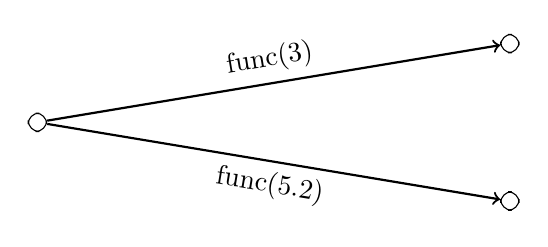
\begin{tikzpicture}[rectangle,rounded corners]
    \draw node (template) [draw] {\usebox{\codepiece}}
          node (templatea) [draw] at (6cm,+1cm) {\usebox{\codepiecea}}
          node (templateb) [draw] at (6cm,-1cm) {\usebox{\codepieceb}};
    \draw[->,thick] (template) -- (templatea) node [above,midway,sloped] {func(3)};
    \draw[->,thick] (template) -- (templateb) node [below,midway,sloped] {func(5.2)};
  \end{tikzpicture}
\end{frame}

\begin{frame}[fragile]
  \frametitle{Templates}
  \begin{block}{Arguments}
    \begin{itemize}
    \item can be a class, 
    \item you can have several
    \item last ones can have a default value
    \end{itemize}
  \end{block}
  \begin{cppcode*}{}
    template<class KeyType=int, class ValueType=KeyType>
    struct Map {
      void set(KeyType &key, ValueType value);
      ValueType get(KeyType &key);
    }

    Map<std::string, int> m1;
    Map<float> m2;   // Map<float, float>
    Map<> m3;        // Map<int, int>
  \end{cppcode*}
\end{frame}

\begin{frame}[fragile]
  \frametitle{Templates implementation}
  \begin{cppcode*}{}
    template<class KeyType=int, class ValueType=KeyType>
    struct Map {
      void set(KeyType &key, ValueType value);
      ValueType get(KeyType &key);
    }

    template<class KeyType, class ElementType>
    void Map<KeyType, ElementType>::set
       (KeyType &key, ValueType value) {
      ...
    }

    template<class KeyType, class ElementType>
    ValueType Map<KeyType, ElementType>::get(KeyType &key) {
      ...
    }
  \end{cppcode*}
\end{frame}

\begin{frame}[fragile]
  \frametitle{Templates}
  \begin{block}{Specialization}
    templates can be specialized for given values of their parameter
  \end{block}
  \begin{cppcode*}{}
    template<unsigned int N> struct Polynom {
      Polynom(float radius);
      float perimeter();
      float m_radius;
    };
    
    template<>
    struct Polynom<6> {
      Polynom(float radius);
      float perimeter() {return 6*m_radius;};
      float m_radius;
    };
  \end{cppcode*}
\end{frame}

\begin{frame}[fragile]
  \frametitle{The full power of templates}
  \begin{alertblock}{Exercise Time}
    \begin{itemize}
    \item go to code/template
    \item look at the OrderedVector code
    \item compile and run test.cpp. See the ordering
    \item modify test.cpp and reuse OrderedVector with Complex
    \item improve OrderedVector to template the ordering
    \item test reverse ordering of strings (from the last letter)
    \item test manhattan order with complex type
    \item check the implementation of Complex
    \item try ordering complex of complex
    \end{itemize}
  \end{alertblock}
\end{frame}

\subsection[STL]{The STL}

\begin{frame}[fragile]
  \frametitle{The Standard Template Library}
  \begin{block}{What it is}
    \begin{itemize}
    \item A library of standard templates
    \item Eveything you need, or ever dreamed of
      \begin{itemize}
      \item strings, containers, iterators
      \item algorithms, functions, sorters
      \item functors, allocators
      \item ...
      \end{itemize}
    \item Portable
    \item Reusable
    \item Efficient
    \end{itemize}
  \end{block}
  \pause
  \begin{alertblock}{Just use it}
    and adapt it to your needs, thanks to templates
  \end{alertblock}
\end{frame}


\begin{frame}[fragile,label=STLcode]
  \frametitle{STL in practice}
  \begin{cppcode*}{}
    #include <vector>
    #include <algorithm>

    std::vector<int> vi, vr(3);
    vi.push_back(5); vi.push_back(3); vi.push_back(4);

    std::transform(vi.begin(), vi.end(),      // range1
                   vi.begin(),          // start range2
                   vr.begin(),          // start result
                   std::multiplies<int>()); // function

    for(std::vector<int>::iterator it = vr.begin();
        it != vr.end();
        it++) {
      std::cout << *it << " ";
    };
  \end{cppcode*}
\end{frame}

\begin{frame}[fragile]
  \frametitle{STL's concepts}
  \begin{block}{containers}
    \begin{itemize}
    \item a structure containing data
    \item with a given way of handling it
    \item irrespective of
      \begin{itemize}
      \item the data itself (templated)
      \item the memory allocation of the structure (templated)
      \item the algorithms that may use the structure
      \end{itemize}
    \item examples
      \begin{itemize}
      \item string
      \item list, vector, deque
      \item map, set, multimap, multiset, hash\_map, hash-set, ...
      \item stack, queue, priority\_queue
      \end{itemize}
    \end{itemize}
  \end{block}
\end{frame}

\begin{frame}[fragile]
  \frametitle{STL's concepts}
  \begin{block}{iterators}
    \begin{itemize}
    \item generalization of pointers
    \item allowing iteration over some data
    \item irrespective of
      \begin{itemize}
      \item the container used (templated)
      \item the data itself (container is templated)
      \item the consumer of the data (templated algorithm)
      \end{itemize}
    \item examples
      \begin{itemize}
      \item iterator
      \item reverse\_iterator
      \item const\_iterator
      \end{itemize}
    \end{itemize}
  \end{block}
\end{frame}

\begin{frame}[fragile]
  \frametitle{STL's concepts}
  \begin{block}{algorithms}
    \begin{itemize}
    \item implementation of an algorithm working on data
    \item with a well defined behavior (defined complexity)
    \item irrespective of
      \begin{itemize}
      \item the data handled
      \item the container where data live
      \item the iterator used to go through data
      \end{itemize}
    \item examples
      \begin{itemize}
      \item for\_each, find, find\_if, count, count\_if, search
      \item copy, swap, transform, replace, fill, generate
      \item remove, remove\_if
      \item unique, reverse, rotate, random, partition
      \item sort, partial\_sort, merge, min, max
      \item lexicographical\_compare, iota, accumulate, partial\_sum
      \end{itemize}
    \end{itemize}
  \end{block}
\end{frame}
      
\begin{frame}[fragile]
  \frametitle{STL's concepts}
  \begin{block}{functions / functors}
    \begin{itemize}
      \item generic utility functions/functors
      \item mostly useful to be passed to STL algorithms
    \item implemented independently of
      \begin{itemize}
      \item the data handled (templated)
      \item the context (algorithm) calling it
      \end{itemize}
    \item examples
      \begin{itemize}
      \item plus, minus, multiply, divide, modulus, negate
      \item equal\_to, less, greater, less\_equal, ...
      \item logical\_and, logical\_or, logical\_not
      \item identity, project1st, project2nd
      \item binder1st, binder2nd, unary\_compose, binary\_compose
      \end{itemize}
    \end{itemize}
  \end{block}
\end{frame}

\againframe{STLcode}

\begin{frame}[fragile]
  \frametitle{More complex STL code}
  \begin{cppcode}
    // Finds the first element in a list that lies in
    // the range from 1 to 10.
    list<int> L;
    ...
    list<int>::iterator in_range = 
      find_if(L.begin(), L.end(),
              compose2(logical_and<bool>(),
                       bind2nd(greater_equal<int>(), 1),
                       bind2nd(less_equal<int>(), 10)));

    // Computes sin(x)/(x + DBL_MIN) for elements of a range.
    transform(first, last, first,
              compose2(divides<double>(),
                       ptr_fun(sin),
                       bind2nd(plus<double>(), DBL_MIN)));
  \end{cppcode}
\end{frame}

\begin{frame}[fragile]
  \frametitle{Welcome to lego programming !}
  \begin{block}{}
    \pgfdeclareimage[height=0.5cm]{AtlasLego}{AtlasLego.jpg}
    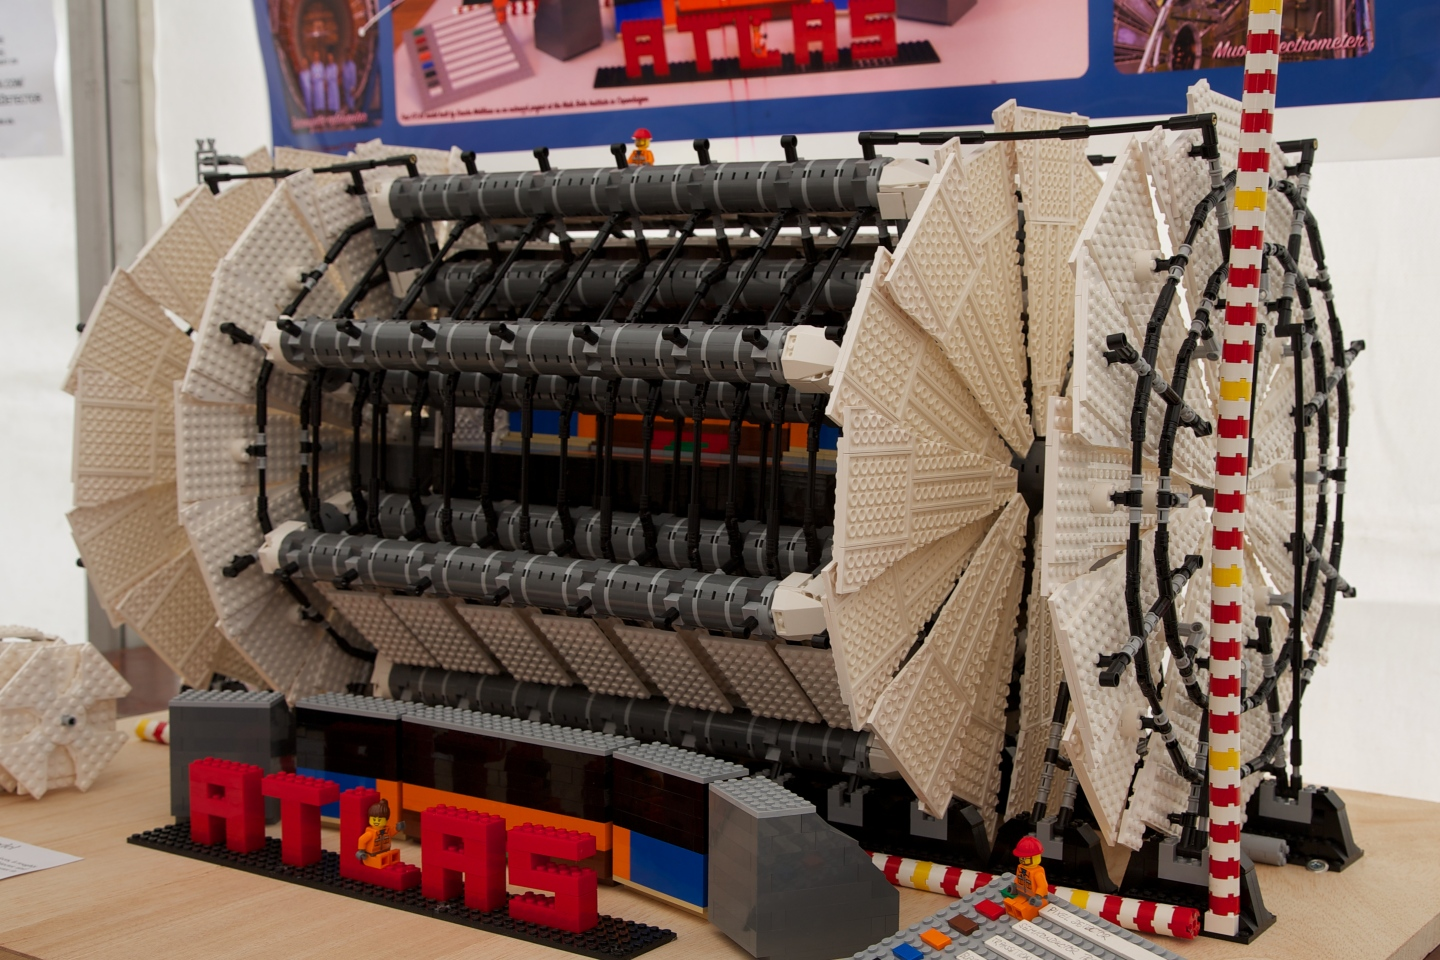
\includegraphics[width=\linewidth]{AtlasLego}
  \end{block}
\end{frame}

\begin{frame}[fragile]
  \frametitle{Using the STL}
  \begin{alertblock}{Exercise Time}
    \begin{itemize}
    \item go to code/stl
    \item look at the non STL code in test.nostl.cpp 
      \begin{itemize}
        \item it creates a vector of ints at regular intervals
        \item it randomizes them
        \item it computes differences between consecutive ints
        \item and the mean and variance of it
      \end{itemize}
    \item open test.cpp and complete the ``translation'' to STL
    \item see how easy it is to reuse the code with complex numbers
    \end{itemize}
  \end{alertblock}
\end{frame}

\begin{frame}[fragile]
  \frametitle{Using the STL}
  \begin{alertblock}{Some last warning}
    You may find the STL quite difficult to use.
    \begin{itemize}
    \item template syntax is simply awful
    \item it is hard to debug (compilers spit out mostly garbage)
    \item the standard is not well defined (SGI vs \cpp98 vs \cpp11)
    \end{itemize}
    However, this has improved a lot with \cpp11
  \end{alertblock}
\end{frame}

\subsection[Tools]{Useful tools}

\begin{frame}[fragile]
  \frametitle{\cpp editor}
  \begin{block}{Choose it wisely}
    \begin{itemize}
    \item it can improve dramatically your efficiency by
      \begin{itemize}
      \item coloring the code for you to ``see'' the structure
      \item helping indenting properly
      \item allowing you to navigate easily in the source tree
      \item helping for compilation/debugging
      \end{itemize}
    \end{itemize}
  \end{block}
  \begin{block}{A few tools}
    \begin{description}
    \item[\href{http://www.microsoft.com/}{\beamergotobutton{Visual Studio}}]
      the Microsoft way
    \item[\href{https://www.eclipse.org/}{\beamergotobutton{Eclipse}}]
      similar, but open source and portable
    \item[\href{https://netbeans.org/features/cpp/}{\beamergotobutton{NetBeans}}]
      similar again, also portable
    \item[\href{http://www.gnu.org/software/emacs/}{\beamergotobutton{Emacs}}]
      the expert way. Extremely powerful. Programmable \\
      It is to IDEs what latex is to PowerPoint
    \end{description}
    Choosing one is mostly a matter of taste
  \end{block}
\end{frame}


\begin{frame}[fragile]
  \frametitle{Code management tool}
  \begin{alertblock}{Please use one !}
    \begin{itemize}
    \item even locally
    \item even on a single file
    \item even if you are the only commiter
    \end{itemize}
    It will soon save your day
  \end{alertblock}
  \begin{block}{A few tools}
    \begin{description}
    \item[\href{http://git-scm.com/}{\beamergotobutton{git}}]
      THE best choice. Fast, light, easy to use
    \item[\href{http://mercurial.selenic.com/}{\beamergotobutton{mercurial}}]
      the main alternative
    \item[\href{http://bazaar.canonical.com/en/}{\beamergotobutton{Bazzar}}]
      another alternative
    \item[svn]
      historical, not distributed - DO NOT USE
    \item[CVS]
      archeological, not distributed - DO NOT USE
    \end{description}
  \end{block}
\end{frame}

\begin{frame}[fragile]
  \frametitle{GIT crash course}
  \begin{minted}[gobble=4]{text}
    # mkdir myProject; cd myProject; git init
    Initialized empty Git repository in /tmp/myProject/.git/

    # vim file.cpp; vim file2.cpp
    # git add file.cpp file2.cpp
    # git commit -m "commiting first 2 files"
    [master (root-commit) c481716] commiting first 2 files
    ...

    # git log --oneline
    d725f2e Better STL test
    f24a6ce Reworked examples + added stl one
    bb54d15 implemented template part
    ...

    # git diff f24a6ce bb54d15
  \end{minted}
\end{frame}


\begin{frame}[fragile]
  \frametitle{The compiling chain}
  \center
  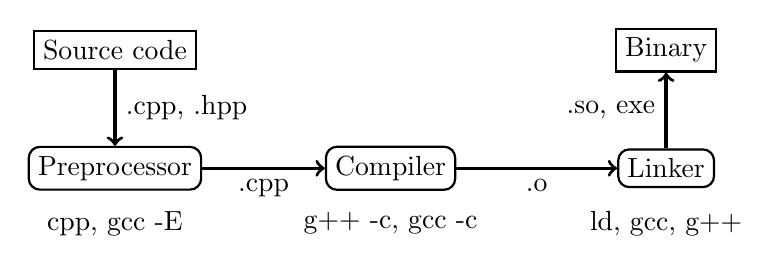
\begin{tikzpicture}
    \draw[thick] node (code) at(0,0) [rectangle,draw] {Source code}
                 node (cpp) at(0, -1.5cm) [rectangle,rounded corners,draw] {Preprocessor}
                 node (gcc) at(3.5cm,-1.5cm) [rectangle,rounded corners,draw] {Compiler}
                 node (ld) at(7cm,-1.5cm) [rectangle,rounded corners,draw] {Linker}
                 node (bin) at(7cm,0) [rectangle,draw] {Binary}
                 node at(0, -2.2cm) {cpp, gcc -E}
                 node at(3.5cm, -2.2cm) {g++ -c, gcc -c}
                 node at(7cm, -2.2cm) {ld, gcc, g++};
    \draw[very thick,->] (code) -- (cpp) node [midway,right] {.cpp, .hpp};
    \draw[very thick,->] (cpp) -- (gcc) node [midway,below] {.cpp};
    \draw[very thick,->] (gcc) -- (ld) node [midway,below] {.o};
    \draw[very thick,->] (ld) -- (bin) node [midway,left] {.so, exe};
  \end{tikzpicture}
  \begin{block}{The steps}
    \begin{description}
    \item[cpp]
        the preprocessor \\
        handles the \# directives (macros, includes) \\
        creates ``complete'' source code
    \item[g++]
        the compiler \\
        creates assembly code from \cpp code
    \item[ld]
        the linker \\
        links several binary files into libraries and executables
    \end{description}
  \end{block}
\end{frame}

\begin{frame}[fragile]
  \frametitle{Compilers}
  \begin{block}{Available tools}
    \begin{description}
    \item[\href{http://gcc.gnu.org/}{\beamergotobutton{gcc}}]
        the most common and most used\\
        free and open source
    \item[\href{http://clang.llvm.org/}{\beamergotobutton{clang}}]
        drop-in replacement of gcc \\
        better output and error reporting \\
        free and open source
    \item[\href{http://software.intel.com/en-us/intel-compilers}{\beamergotobutton{icc}}]
        the intel compiler \\
        proprietary \\
        optimized for Intel hardware
    \item[\href{http://www.microsoft.com/}{\beamergotobutton{Visual \cpp}}]
      the Windows way
    \end{description}
  \end{block}
  \begin{alertblock}{My prefered choice today}
    \begin{itemize}
      \item \alert{clang} for its error reporting
      \item \alert{gcc} is not far and tries to catch up
    \end{itemize}
  \end{alertblock}
\end{frame}

\begin{frame}[fragile]
  \frametitle{Useful compiler options (gcc/clang)}
  \begin{block}{Get more warnings}
    \begin{description}
      \item[-Wall -Wextra] the way to get all warnings
      \item[-Werror] the way to force yourself to look at warnings
    \end{description}
  \end{block}
  \begin{block}{Around optimization}
    \begin{description}
      \item[-g] add debug symbols
      \item[-O0, -O2] 0 = no optimization, -O2 = optimized
    \end{description}
  \end{block}
  \begin{block}{Compilation environment}
    \begin{description}
      \item[\texttt{-I} \textless{}path\textgreater] where to find header files
      \item[\texttt{-L} \textless{}path\textgreater] where to find libraries
      \item[\texttt{-l} \textless{}name\textgreater] link with libname.so
      \item[\texttt{-E / -c}] stop after preprocessing / compilation
    \end{description}
  \end{block}
\end{frame}

\begin{frame}[fragile]
  \frametitle{Makefiles}
  \begin{block}{Why to use them}
    \begin{itemize}
    \item an organized way of describing building steps
    \item avoids a lot of typing
    \end{itemize}
  \end{block}
  \begin{block}{Several implementations}
    \begin{itemize}
    \item raw Makefiles : suitable for small projects
    \item cmake : portable, the current best choice
    \item automake : portable but complex
      \end{itemize}
  \end{block}
  \begin{minted}{makefile}
    test : test.cpp libpoly.so
        $(CXX) -Wall -Wextra -o $@ $^
    libpoly.so: Polygons.cpp
        $(CXX) -Wall -Wextra -shared -fPIC -o $@ $^
    clean:
        rm -f *o *so *~ test test.sol
  \end{minted}
\end{frame}

\begin{frame}[fragile]
  \frametitle{Compiler chain}
  \begin{alertblock}{Exercise Time}
    \begin{itemize}
    \item go to code/polymorphism
    \item preprocess Polygons.cpp (cpp or gcc -E -o output)
    \item compile Polygons.o and test.o (g++ -c -o output)
    \item use nm to check symbols
    \item see link statement using g++ -v
    \item see library dependencies with ldd
    \item look at the Makefile
    \item try make clean; make
    \end{itemize}
  \end{alertblock}
\end{frame}


\begin{frame}[fragile]
  \frametitle{Debugging}
  \begin{alertblock}{The problem}
    \begin{itemize}
      \item everything compiles fine (no warning)
      \item but crashes at run time
      \item no error message, no clue
    \end{itemize}
  \end{alertblock}
  \pause
  \begin{block}{The solution : debuggers}
    \begin{itemize}
    \item dedicated program able to stop execution at any time
    \item and show you where you are and what you have
    \end{itemize}
  \end{block}
  \pause
  \begin{block}{Existing tools}
    \begin{description}
    \item[\href{http://www.sourceware.org/gdb/}{\beamergotobutton{gdb}}]
      THE main player
    \item[\href{http://lldb.llvm.org/}{\beamergotobutton{lldb}}]
      the debugger coming with clang \\
      still young, no stable version
    \item[\href{http://software.intel.com/en-us/articles/idb-linux}{\beamergotobutton{idb}}]
      the intel debugger, proprietary
    \end{description}
  \end{block}
\end{frame}

\begin{frame}[fragile]
  \frametitle{gdb crash course}
  \begin{block}{start gdb}
    \begin{itemize}
    \item gdb \textless{}program\textgreater
    \item gdb \textless{}program\textgreater \textless{}core file\textgreater
    \end{itemize}
  \end{block}
  \begin{block}{inspect state}
    \begin{description}
    \item[bt] prints a backtrace
    \item[print \textless{}var\textgreater] prints current content of the variable
    \item[list] show code around current point
    \item[up/down] go up or down in call stack
    \end{description}
  \end{block}
  \begin{block}{breakpoints}
    \begin{description}
    \item[break \textless{}function\textgreater] puts a breakpoint on function entry
    \item[break \textless{}file\textgreater:\textless{}line\textgreater] puts a breakpoint on that line
    \end{description}
  \end{block}
\end{frame}

\begin{frame}[fragile]
  \frametitle{gdb}
  \begin{alertblock}{Exercise Time}
    \begin{itemize}
    \item go to code/debug
    \item compile, run, see the crash
    \item run it in gdb
    \item inspect backtrace, variables
    \item find problem and fix bug
    \item try stepping, breakpoints
    \item use -Wall -Wextra and see warning
    \end{itemize}
  \end{alertblock}
\end{frame}



\begin{frame}[fragile]
  \frametitle{The valgrind family}
  \begin{block}{Valgrind fundamentals}
    \begin{itemize}
    \item valgrind is a framework for different tools
    \item a processor simulator allowing checks in between instructions
    \item slow (10-50 times slower than normal execution)
    \item easy to use : ``valgrind \textless{}your executable\textgreater''
      \begin{itemize}
      \item no recompilation
      \item better with -g -O0, but not strictly needed
      \end{itemize}
    \item it is free and open source
    \end{itemize}
  \end{block}
  \pause
  \begin{block}{Main tools}
    \begin{description}
      \item[memcheck] a memory checker (default tool) and leak detector
      \item[callgrind] a call graph builder
      \item[helgrind] a race condition detector
    \end{description}
  \end{block}
\end{frame}

\begin{frame}[fragile]
  \frametitle{memcheck}
  \begin{block}{}
    \begin{itemize}
      \item keeps track of all memory allocations and deallocations
      \item is able to detect accesses to non allocated memory
      \item and even tell you when it was deallocated if it was
      \item or what it the closest array in case of overflow
      \item is able to list still allocated memory when program exits\\
        (memory leaks detection)
    \end{itemize}
  \end{block}
\end{frame}

\begin{frame}[fragile]
  \frametitle{valgrind}
  \begin{alertblock}{Exercise Time}
    \begin{itemize}
    \item go to code/valgrind
    \item compile, run, it should work
    \item run with valgrind, see the problem
    \item fix the problem
      \vspace{.3cm}
    \item go back to the code/debug exercise
    \item check it with valgrind
    \item analyze the issue, see that the variance was biaised
    \item fix the issue
    \end{itemize}
  \end{alertblock}
\end{frame}

\begin{frame}[fragile]
  \frametitle{memcheck}
  \begin{alertblock}{Exercise Time}
    \begin{itemize}
    \item go to code/memcheck
    \item compile, run, it should work
    \item run with valgrind, see LEAK summary
    \item run with -{}-leak-check=full to get details
    \item analyze and correct it
    \end{itemize}
  \end{alertblock}
\end{frame}

\begin{frame}[fragile]
  \frametitle{callgrind and kcachegrind}
  \begin{block}{callgrind}
    \begin{itemize}
      \item keeps track of all function calls
      \item and time spent in each function
      \item build statistics on calls, CPU usages and more
      \item outputs flat statistics file, quite unreadable
    \end{itemize}
  \end{block}
  \begin{block}{kcachegrind}
    \begin{itemize}
      \item a gui exploiting statistics built by callgrind
      \item able to browse graphically the program calls
      \item able to ``graph'' CPU usage on the program structure
    \end{itemize}
  \end{block}
\end{frame}

\begin{frame}[fragile]
  \frametitle{callgrind}
  \begin{alertblock}{Exercise Time}
    \begin{itemize}
    \item go to code/callgrind
    \item compile, run, it will be slow
    \item change nb iterations to 20
    \item run with valgrind -{}-tool=callgrind
    \item look at output with kcachegrind
    \item change fibo call to fibo2
    \item observe the change in kcachegrind
    \end{itemize}
  \end{alertblock}
\end{frame}

\begin{frame}[fragile]
  \frametitle{helgrind}
  \begin{block}{}
    \begin{itemize}
      \item keeps track of all pthreads activity
      \item in particular keeps track of all mutexes
      \item builds a graph of dependencies of the different actions
      \item works on the resulting graph to detect:
        \begin{itemize}
        \item possible dead locks
        \item possible data races
        \end{itemize}
    \end{itemize}
  \end{block}
  \pause
  \begin{alertblock}{}
    Note the ``possible''. It finds future problems !
  \end{alertblock}
\end{frame}

\begin{frame}[fragile]
  \frametitle{helgrind}
  \begin{alertblock}{Exercise Time}
    \begin{itemize}
    \item go to code/helgrind
    \item compile, run
    \item check it with valgrind. See strange behavior \\
      but no explanation
    \item check it with valgrind -{}-tool=helgrind
    \item understand issue and fix
    \end{itemize}
  \end{alertblock}
\end{frame}


\begin{frame}[fragile]
  \frametitle{Static analysis}
  \begin{alertblock}{The problem}
    \begin{itemize}
    \item all the tools discussed so far work on binaries
    \item they analyze the code being run
    \item so there is a coverage problem (e.g. for error cases)
    \end{itemize}
  \end{alertblock}
  \pause
  \begin{block}{A (partial) solution : analyzing the source code}
    \begin{itemize}
    \item build a graph of dependencies of the calls
    \item use graph tools to detect potential memory corruptions,
      memory leaks ot missing initializations
    \end{itemize}
  \end{block}
  \pause
  \begin{block}{Existing tools}
    \begin{description}
    \item[\href{http://www.coverity.com/}{\beamergotobutton{Coverity}}]
      proprietary tool, the most complete
    \item[\href{http://cppcheck.sourceforge.net/}{\beamergotobutton{cppcheck}}]
      free and opensource, but less complete
    \item[\href{http://clang-analyzer.llvm.org/}{\beamergotobutton{scan-build}}]
      the clang source analyzer, still young
    \end{description}
  \end{block}
\end{frame}

\begin{frame}[fragile]
  \frametitle{cppcheck}
  \begin{alertblock}{Exercise Time}
    \begin{itemize}
    \item go to code/cppcheck
    \item compile, run, see that it works
    \item use valgrind : no issue
    \item use cppcheck, see the problem
    \item analyze the issue, and fix it
    \item bonus : understand why valgrind did not complain \\
      and how the standard deviation was biased \\
      hint : try to use malloc to create v
    \end{itemize}
  \end{alertblock}
\end{frame}
